\chapter{Os Softwares}
	\label{capituloSoftwares}

	Ao decorrer deste trabalho, fora o software que implementa a técnica de reconstrução descrita nesta monografia, foi sendo necessário que técnicas adjuntas à estudada aqui também fossem implementadas em softwares a fim de facilitar comprovações de resultados e automatizações de tarefas auxiliares ao projeto; além de agregar determinada riqueza de esforço e de ferramentas a este trabalho de conclusão de curso.
	
	A seguir são apresentados os exemplos mais representativos dos softwares desenvolvidos ao longo do projeto.
	
	\section{Aplicativo de detecção de retas}
		\label{appDeteccaoRetas}
		Tanto para auxiliar na detecção automática dos segmentos de reta do sistema de coordenadas de referência quanto dos pontos (interseção de segmentos de reta) de interesse à reconstrução. Foi desenvolvido um aplicativo para a obtenção de parâmetros analíticos de retas apresentadas em uma região de uma imagem digital.
		
		As linhas inferidas como interessantes, por serem representadas através da rasterização - processo de conversão da representação vetorial para a matricial \cite{compGrafTeoPrat} - precisaram sofrer um processo de regressão linear a fim de se obter uma aproximação dos parâmetros geométricos analíticos de sua formação. A regressão linear executada para a obtenção dos coeficientes angular e linear das retas de interesse se deu através do método dos mínimos quadrados.
	
	O Métodos dos Mínimos Quadrados é uma técnica de regressão linear que busca ajustar corretamente coeficientes de uma curva algébrica de forma que estes minimizem o somatório do quadrado da diferença entre os valores dos dados reais e os valores estimados, minimizando o erro de aproximação.
	
	Com uma interface apropriada, pôde-se carregar uma imagem e, através da demarcação manual de uma região de interesse na mesma (demarcada por um retângulo vermelho), pontos da possível linha foram detectados pela sua cor preta e submetidos ao método dos mínimos quadrados (figura \ref{figMinQuadInterface}).
	
	Após a aproximação são exibidos, na parte superior da janela, os coeficientes encontrados e é plotada, sobre a imagem, a reta encontrada.
	
	\begin{figure}[!htb]
		\centering
		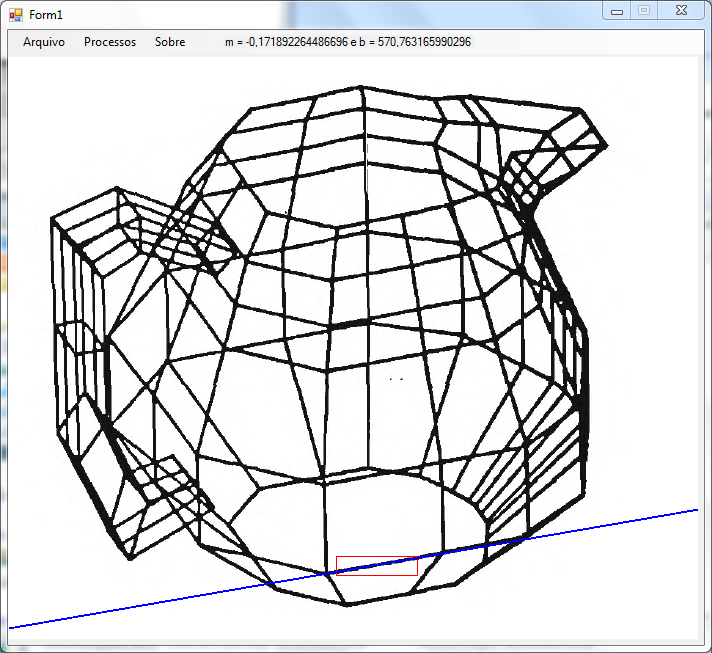
\includegraphics[height=6cm]{imagens/printAppMinimosQuadrados.png}
		\caption{O programa de regressão de rasterização com uma aproximação de exemplo}
		\label{figMinQuadInterface}
	\end{figure}

	Posteriormente, os coeficientes encontrados foram submetidos ao programa Microsoft Mathematics\textregistered  comprovando que os valores encontrados são coerentes (figura \ref{mathematics}). Note que, como o sentido de orientação dos pontos da imagem (de cima para baixo) é inverso ao do plano cartesiano (de baixo para cima) o aspecto da reta em relação ao aspecto da linha é invertido.
	
	\begin{figure}[!htb]
		\centering
		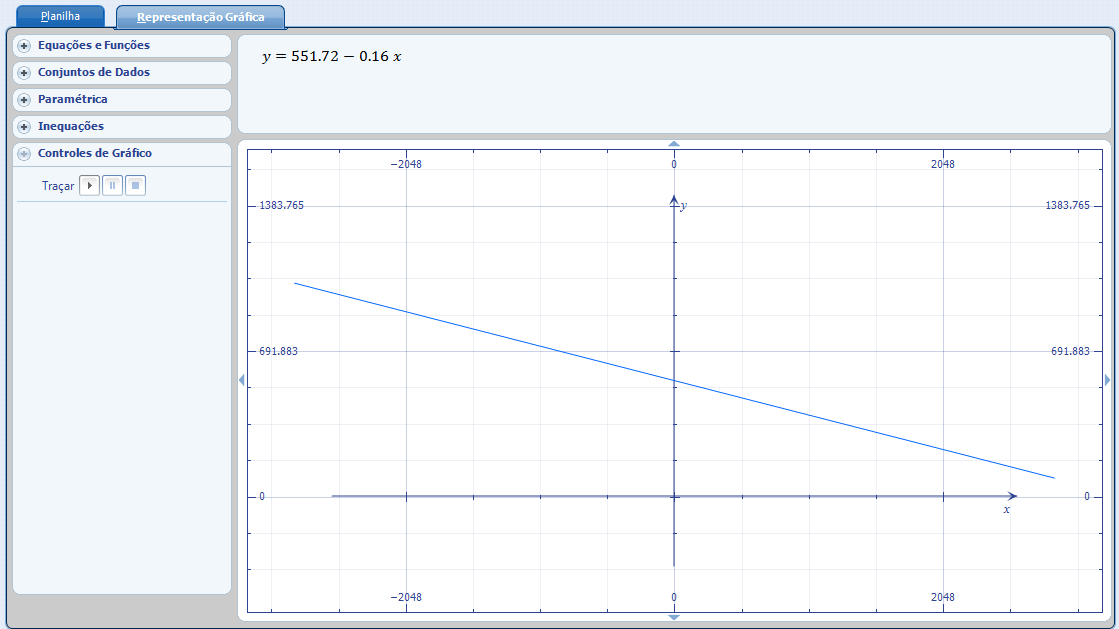
\includegraphics[height=5cm]{imagens/mathematics1.png}
		\caption{Reta analítica correspondente à linha da região demarcada na figura \ref{figMinQuadInterface}}
		\label{mathematics}
	\end{figure}
	
	Com esta técnica se obteve uma possibilidade de automatização da busca de elementos de interesse nas imagens estudadas.
	
	Este aplicativo está disponível em \url{https://github.com/ivancezanne/TCC/tree/master/App_MinimosQuadrados}.
	
	\section{Aplicativo de Projeção 3D}
		\label{app3D}
		
		Tendo em vista que o resultado deste trabalho é gerar malhas 3D, um aplicativo (figura \ref{imagemApp3D}), baseado na descrição presente em \cite{compGraphsPrincPrat3ed} e capaz de interpretar aquivos PLY \cite{ply}, foi desenvolvido. Mesmo apresentando uma limitação quanto a definições de usuário em relação a cores e normais de faces, a utilidade deste aplicativo no contexto deste trabalho foi notável.
		
		\begin{figure}[!htb]
			\centering
			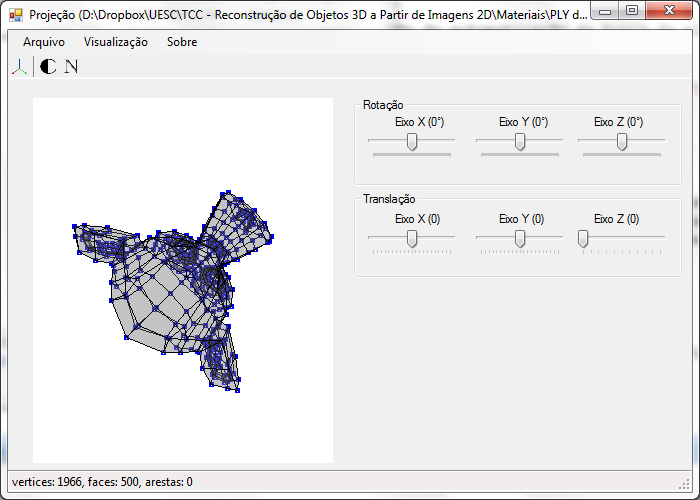
\includegraphics[height=5cm]{imagens/printApp3D.png}
			\caption{Aplicativo de projeção 3D com a famosa malha Suzanne}
			\label{imagemApp3D}
		\end{figure}
		
		Além da projeção da malha 3D descrita em um arquivo PLY de entrada, este aplicativo possibilita manipulações geométricas na malha (translação e rotação, apenas) e algoritmos prontos de normalização (alteração proporcional das dimensões para o máximo de 1 unidade de medida) e centralização (translação do baricentro da malha à origem do espaço 3D).
		
		Como auxílios visuais o aplicativo também permite escolher quais elementos da malha deverão ser projetados à visualização (figura \ref{imagemApp3DRenderizar}) e alterar as cores dos elementos que compõem a malha (figura \ref{imagemApp3DCores}).
		
		\begin{figure}[!htb]
			\centering
			\subfloat[Menu onde se escolhe quais elementos da malha serão renderizados]{
				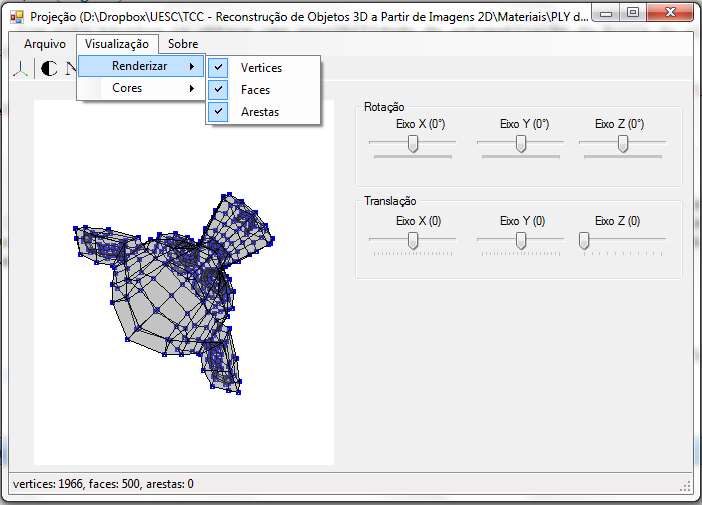
\includegraphics[height=5cm]{imagens/printApp3D-renderizar.png}
				\label{imagemApp3DRenderizar}
			}
			\quad
			\subfloat[Menu onde se pode alterar as cores dos elementos da malha]{
				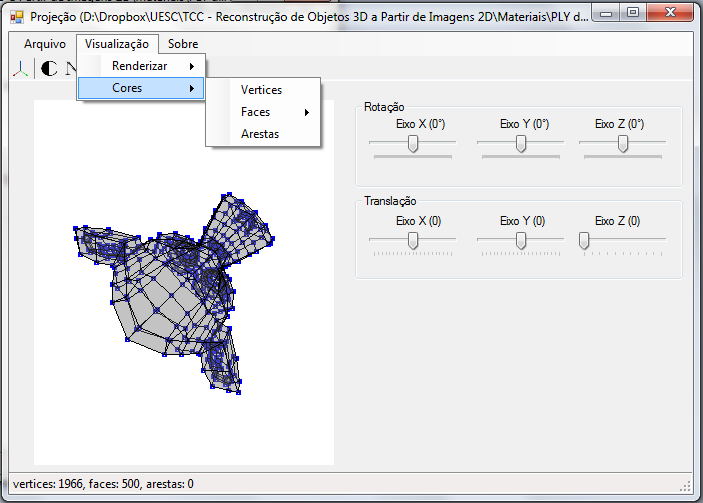
\includegraphics[height=5cm]{imagens/printApp3D-cores.png}
				\label{imagemApp3DCores}
			}
			\caption{Opções adicionais do aplicativo de projeção 3D de auxílio à visualização}
			\label{imagemApp3DAuxiliosVisuais}
		\end{figure}
		
		Por muitas vezes as funcionalidades implementadas neste aplicativo o fizeram preferível, na visualização de resultados deste trabalho, em relação ao \textit{software} MeshLab.
		
		Este aplicativo pode ser encontrado em \url{https://github.com/ivancezanne/TCC/tree/master/App_Projecao}.
		
	\section{Aplicativo de Reconstrução}
		\label{appReconstrucao}
		
		A técnica de reconstrução deste trabalho (capítulo \ref{capituloReconstrucao}) foi implementada através de um \textit{software} (figura \ref{printAppReconstrucao}) que, com forte auxílio visual, busca otimizar a reconstrução almejada.
		
		\begin{figure}[!htb]
			\centering
			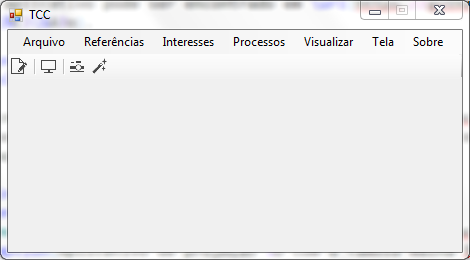
\includegraphics[height=4cm]{imagens/printAppReconstrucao.png}
			\caption{Tela inicial do aplicativo de reconstrução}
			\label{printAppReconstrucao}
		\end{figure}
		
		Inicialmente, o software necessita que uma imagem seja aberta em sua interface para que as demais funcionalidades sejam disponibilizadas. Com uma imagem carregada (que já é aberta com um conjunto de referências arbitrário), a demarcação de pontos de referência e de interesse (capítulo \ref{capituloReconstrucao}) pode ser feita através de \textit{clicks} na região desejada da imagem (figura \ref{printAppReconstrucaoDemarcacao}).
		
		\begin{figure}[!htb]
			\centering
			\subfloat[Interface apenas com uma imagem incial]{
				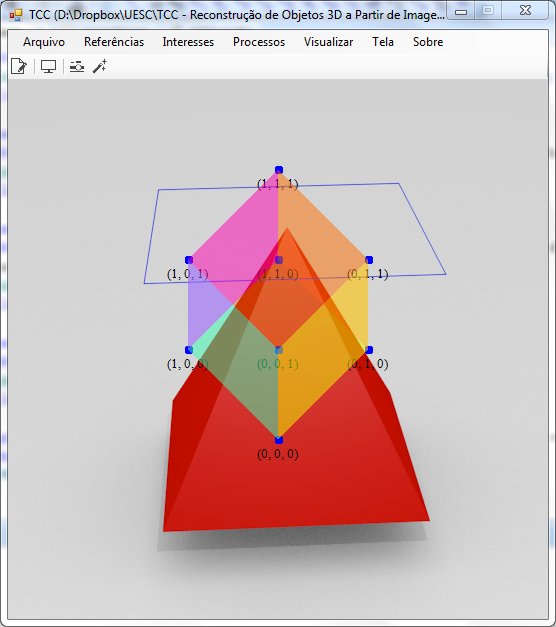
\includegraphics[height=4cm]{imagens/printAppReconstrucaoInicio.png}
				\label{AppReconstrucaoInicio}
			}
			\enskip
			\subfloat[Após o \textit{click}, um \textit{prompt} solicita dados acerca do ponto]{
				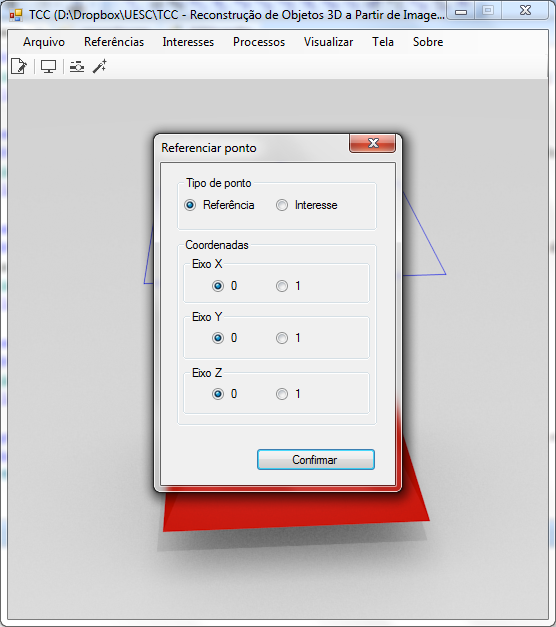
\includegraphics[height=4cm]{imagens/printAppReconstrucaoPrompt.png}
				\label{AppReconstrucaoPrompt}
			}
			\enskip
			\subfloat[Pelos \textit{radio buttons}, o mesmo \textit{prompt} é utilizado para catalogar pontos de referência e de interesse]{
				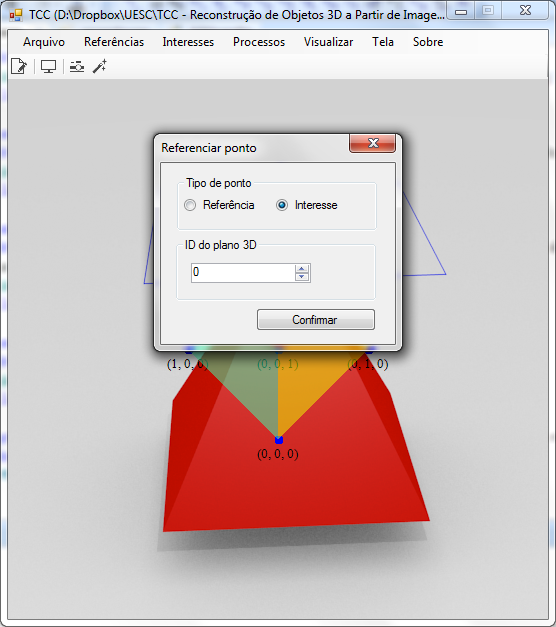
\includegraphics[height=4cm]{imagens/printAppReconstrucaoPromptInteresse.png}
				\label{AppReconstrucaoPromptInteresse}
			}
			\enskip
			\subfloat[Uma cena completamente catalogada]{
				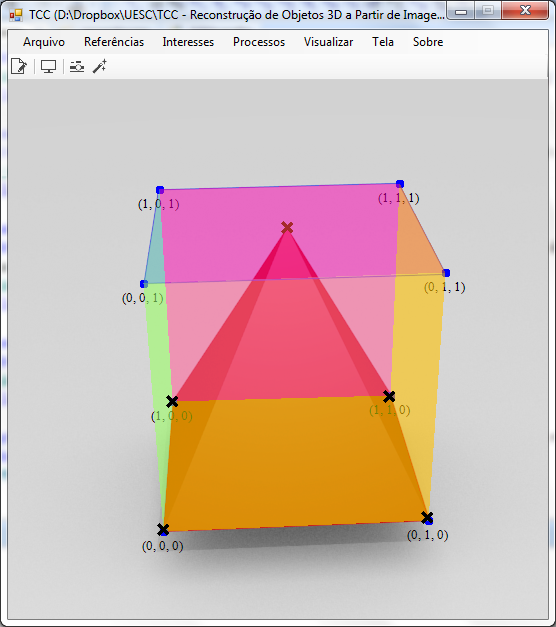
\includegraphics[height=4cm]{imagens/printAppReconstrucaoPronto.png}
				\label{AppReconstrucaoPronto}
			}
			\caption{Utilização da interface para a demarcação de pontos de referência e interesse}
			\label{printAppReconstrucaoDemarcacao}
		\end{figure}
		
		Após o completo fornecimento de dados para a reconstrução, é necessário que se execute a calibração de câmera e só então a reconstrução será possível de ser executada. Para a implementação da calibração foi utilizada o método de cálculo de autovalores e autovetores, baseado no algoritmo QR, da biblioteca ALGLIB Free Edition v3.8.2 para linguagem C\#.
		
		Ao início da reconstrução, os dados descritos no capítulo \ref{capituloReconstrucao} (tolerância projetiva, incremento e critério de convergência) são requisitados pelo software e seu fornecimento é obrigatório ao usuário (figura \ref{printAppReconstrucaoReconstrucao}).
		
		\begin{figure}[!htb]
			\centering
			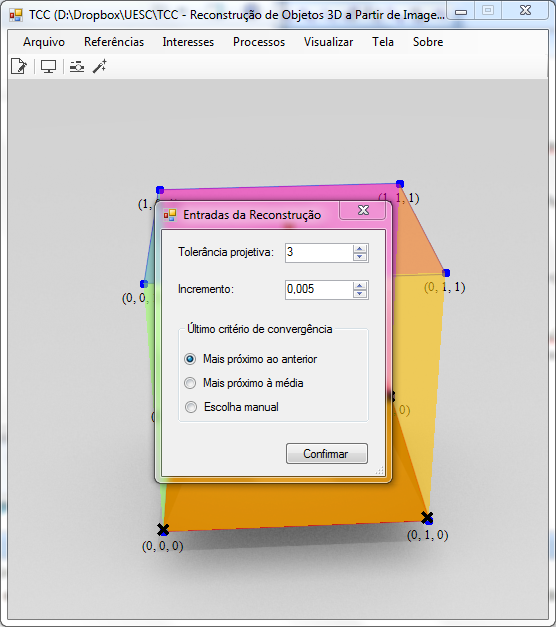
\includegraphics[height=5cm]{imagens/printAppReconstrucaoReconstrucao.png}
			\caption{\textit{Prompt} com dados necessários à reconstrução}
			\label{printAppReconstrucaoReconstrucao}
		\end{figure}
		
		Em adição aos critérios arbitrários de convergência descritos no capítulo \ref{capituloReconstrucao}, o software oferece a possibilidade de escolha manual, pelo usuário, do valor da coordenada Z dentre os que o algoritmo já encontrou como possíveis (figura \ref{printAppReconstrucaoEscolhaManual})
		
		\begin{figure}[!htb]
			\centering
			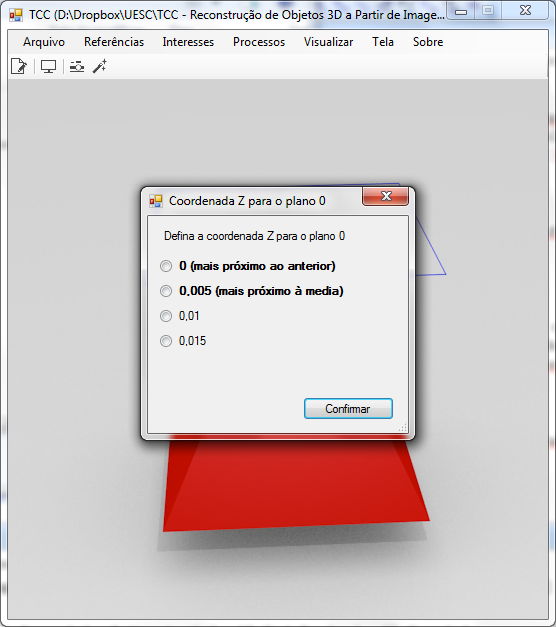
\includegraphics[height=5cm]{imagens/printAppReconstrucaoEscolhaManual.png}
			\caption{\textit{Prompt} para escolha manual da coordenada Z}
			\label{printAppReconstrucaoEscolhaManual}
		\end{figure}
		
		Em posse disto a técnica de reconstrução proposta neste trabalho pode ser executada por qualquer usuário interessado através de um interface adequada. Todavia, ferramentas adicionais como visualização de aproximação após calibração de câmera; salvamento e carregamento de pontos de referência e de interesse através de arquivos; e captura de tela de trabalho foram implementadas tornando o uso do software mais completo e eficiente.
		
		Este aplicativo de reconstrução está disponível em \url{https://github.com/ivancezanne/TCC/tree/master/App_Reconstrucao}.
		